\documentclass[a4paper,12pt]{article}

%% Language and font encodings
\usepackage[english, russian]{babel}
\usepackage[utf8x]{inputenc}
\usepackage{blindtext}
\usepackage[T1]{fontenc}
\usepackage[T2A]{fontenc}
\usepackage[a4paper,top=1.5 cm,bottom=2cm,left=3cm,right=3cm,marginparwidth=1.75cm]{geometry}
%% Useful packages
\usepackage{amsmath, amssymb}
\usepackage{wrapfig}
\usepackage{graphicx}
\usepackage[usenames]{color}
\usepackage[T1]{fontenc}
\usepackage{tikz}
\usetikzlibrary{arrows}
\usetikzlibrary{decorations.pathreplacing}
\usepackage[T2A]{fontenc}
\usepackage{color}
\usepackage{circuitikz} 
\usetikzlibrary{circuits}
\usetikzlibrary{circuits.ee}
\usetikzlibrary{circuits.ee.IEC}
\usetikzlibrary{circuits.logic.IEC}
\graphicspath{{pic/}}
\definecolor{water} {rgb} {0.667, 0.855, 1}
\usepackage{pgfplots}
\usepackage{pgfplotstable}

\title{ИССЛЕДОВАНИЕ РАЗРЕШАЮЩЕЙ СПОСОБНОСТИ МИКРОСКОПА МЕТОДОМ АББЕ}
\date{Работа 4.3.3}
\author{Ляликова Ирина, Б05-911}
\begin{document}
	
	\vspace{0.5 cm}
	\maketitle
	\vspace{0.5 cm}
	
	\textbf{Цель работы:} изучение дифракционного предела разрешения объектива микроскопа.\\
	\vspace{0.3 cm}
	
	\textbf{В работе используются:} лазер; кассета с набором сеток разного
	периода; линзы; щель с микрометрическим винтом; оптический стол
	c набором рейтеров и крепёжных винтов; экран; линейка.\\
	
	\section*{Теоретическое введение} 
	
	\textit{Разрешающей способностью оптического прибора} называют минимальное расстояние $l_{\min}$ между двумя точками в пространстве предметов, изображения которых разрешаются по методу Релея. Эту величину можно рассчитать для лупы и прочих оптических приборов.
	
	\begin{figure}[h]
		\begin{center}
			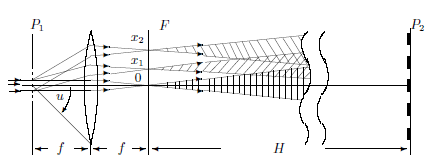
\includegraphics[width = 0.7\textwidth]{433-1.png}
			\caption{Образование изображения в объективе микроскопа.}
		\end{center}
	\end{figure}
	
	Если наблюдения ведутся при внешнем освещении, то когерентные волны рассеивают различные точки предмета. Схема образования изображения представлена на рис. 1.
	
	\section*{Подход Аббе к нахождению разрешающей способности микроскопа}
	Разобьем путь лучей от предмета к изображению на 2 этапа:
	\begin{enumerate}
		\item Картина, возникающая в задней фокальной плоскости $F$ --- \textit{первичное изображение}. 
		\item Первичное изображение --- источник волн $\Rightarrow$. Из этих волн возникает \textit{вторичное изображение}.
	\end{enumerate}
	
	Легко видеть, что первичное изображение представляет собой картину дифракции Фраунгофера. 
	
	\begin{figure}[h]
		\begin{center}
			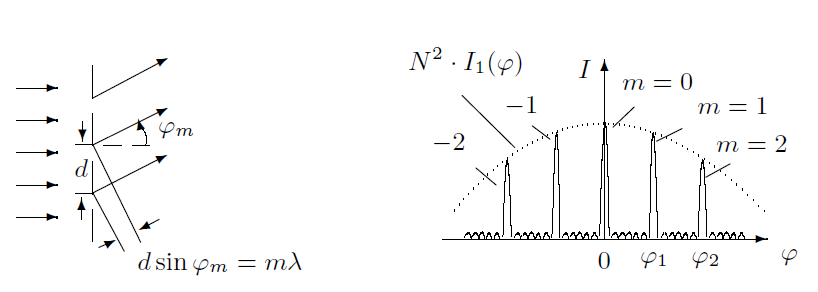
\includegraphics[width = 0.8\textwidth]{433-2.png}
			\caption{Спектр амплитудной решетки}
		\end{center}
	\end{figure}
	При дифракции Фраунгофера на решетке периода $d$ направления $\varphi_m$ максимальной интенсивности определяются из условия 
	\begin{equation}
	d \sin \varphi_m = m \lambda
	\end{equation}
	
	Из рис. 2 легко видеть, что у различных максимумов разные интенсивности.
	В итоге у нас излучение точечных источников на равном расстоянии, отсюда интерференция. 
	
	При таком рассмотрении, из того, что линза конечна следует, что есть дифракционные искажения, так как проходят только те волны, для которых верно 
	\begin{equation}
	\varphi_m < u
	\end{equation}
	
	где $u$ --- \textit{апертурный угол} (см. рис. 1).
	
	\begin{wrapfigure}{r}{0.35\textwidth}
		\begin{center}
			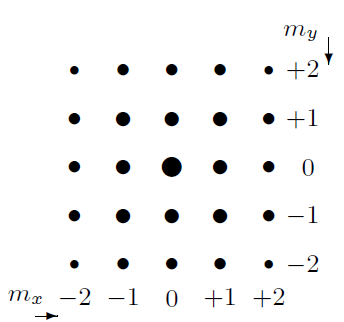
\includegraphics[width = 0.25\textwidth]{433-3.png}
		\end{center}
		\caption{Дифракция Фраунгофера на двумерной решетке}
	\end{wrapfigure}
	
	Если приоткрыть диафрагму и пустить нулевой и один из первых максимумов, то получим периодическую картинку, рассчитаем период. $x_1$ между нулевым и первыми максимумами:
	\begin{equation}
	x_1 \approx f \varphi_1 = f \lambda/d
	\end{equation} 
	
	Ширина интерференционных полос:
	\begin{equation}
	l = \lambda/\omega
	\end{equation} 
	
	где $\omega = x_1/H$ --- угол схождения интерферирующих лучей в точке наблюдения, а $H$ --- расстояние между $F$ и $P_2$. Таким образом, 
	\begin{equation}
	l \approx \lambda H/x_1 = H d/f
	\end{equation}
	
	\begin{equation}
	d' \approx \dfrac{H + f}{f} d
	\end{equation}
	
	Условие разрешения решетки с периодом $d$:
	\begin{equation}
	\sin u \geqslant \lambda/d \Rightarrow 
	\end{equation}
	
	\begin{equation}
	d \geqslant \dfrac{\lambda}{\sin u} \approx \dfrac{\lambda}{D/2f}
	\end{equation}
	Если есть не только 0 максимум, то 
	\begin{equation}
	d \geqslant \dfrac{\lambda}{2 \sin u}
	\end{equation}
	
	У нас решетка двумерная, поэтому мы можем записать все тоже самое в двух осях и получить картину как на рис. 3.
	
	
	\textbf{Экспериментальная установка.} Схема модели проекционного микроскопа приведена на рис. 4. Предметом служат сетки, расположенные в кассете. Смена сеток осуществляется поворотом внешнего кольца кассеты.
	
	\begin{figure}[h]
		\begin{center}
			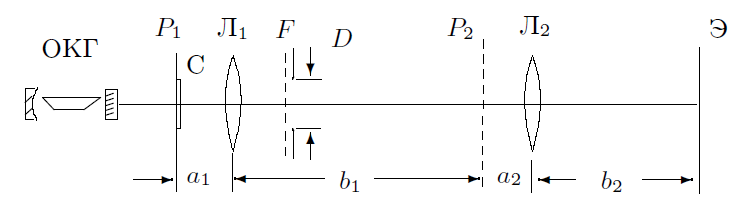
\includegraphics[width = 0.8\textwidth]{433-4.png}
			\caption{Схема установки}
		\end{center}
	\end{figure}
	
	\section*{Ход работы}
	Везде ниже мы работаем с зеленым светом у которого длина волны $\lambda = 532  \text{ нм}$.
	\begin{enumerate}
		\item \textbf{Определение периода решёток по их пространственному спектру.}
		
		
		Соберем установку. Закрепим винтом кассету с двумерными решётками (сетками) вблизи выходного окна лазера так, чтобы в окошке под отверстием с сеткой был виден номер сетки. В каждой кассете 5 различных решёток.
		Вращая наружное кольцо кассеты, получим на удалённом экране дифракционные
		картины для разных сеток. Для определения расстояния между соседними дифракционными максимумами измеряем расстояние между удаленными друг от друга максимумами (горизонтальными или вертикальными) и число промежутков между ними.
		Измерения для шести разных сеток:
		\begin{center}
			\centering\begin{tabular}{|c|c|c|c|c|c|}
				\hline
				№ сетки & 1 & 2 & 3 & 4 & 5 \\ \hline
				$l$, мм & 247$\pm$1 & 260$\pm$1 & 259$\pm$1 & 145$\pm$1 & 177$\pm$1 \\ \hline
				$N$, полос & 7 & 11 & 22 & 24 & 40 \\ \hline
				$\Delta l$, мм & 35,3$\pm$0,1 & 23,66$\pm$0,09 & 11,77$\pm$0,05 & 6,04$\pm$0,04 & 4,42$\pm$0,03 \\ \hline
			\end{tabular}
		\end{center}
		
		Расстояние от сетки до экрана  $H = 133{,}0\pm0{,}5$ см.
		\item \textbf{Определение периода решёток по изображению, увеличенному с помощью модели микроскопа.}
		
		Соберём модель проекционного микроскопа (рис. 4). Длиннофокусная линза Л1 ($f = 110\pm1$ мм) отстоит от сетки на расстоянии чуть большем фокусного, при этом изображение сетки в плоскости получится на расстоянии, в несколько раз превышающем фокусное. С помощью короткофокусной ($F = 25\pm1$ мм) линзы Л2 получаем резкое изображение сетки на экране.
		
		Параметры установки: $a_1 = 155\pm5$ мм, $b_1 + a_2 = 460\pm10$ мм, $b_2 = 715\pm5\text{ мм}$. Так
		как для одной линзы увеличение равно $b/a$, то для всей системы оно составляет $b_1b_2/(a_1a_2)$. Периоды изображений сеток на экране:
		\begin{center}
			\centering\begin{tabular}{|c|c|c|c|c|c|}
				\hline
				№ сетки & 1 & 2 & 3 & 4 & 5 \\ \hline
				$l$, мм & 94$\pm$1 & 84$\pm$1 & 124$\pm$1 & 157$\pm$1 & 150$\pm$1 \\ \hline
				$N$, полос & 50 & 30 & 20 & 14 & 10 \\ \hline
				$\Delta l$, мм & 1,88$\pm$0,02 & 2,80$\pm$0,04 & 6,20$\pm$0,05 & 11,21$\pm$0,07 & 15,0$\pm$0,1 \\ \hline
			\end{tabular}
		\end{center}
	
	\item \textbf{Определение периода решёток по оценке разрешающей способности
		микроскопа.}
		
		Помещаем щелевую диафрагму с микрометрическим винтом в фокальную плоскость $F$ линзы Л1. Определяем для каждой решётки минимальный размер диафрагмы $D$, при котором на экране еще видно изображение сетки (при меньших размерах щели изображение выглядит как одномерная решётка):
		\begin{center}
			\centering\begin{tabular}{|c|c|c|c|c|c|}
				\hline
				№ сетки & 1 & 2 & 3 & 4 & 5 \\ \hline
				$D$, мм & $>4$ & $>4$ & $2{,}0\pm0{,}1$ & $0{,}9\pm0{,}1$ & $0{,}8\pm0{,}1$ \\ \hline
			\end{tabular}
		\end{center}
		
	\item \textbf{Пространственная фильтрация и мультиплицирование.}
	
	Для сетки средних размеров с достаточно крупным вторичным изображением подбираем ширину щели так, чтобы она свободно пропускала максимум нулевого порядка и не пропускала максимумы первого порядка, расположенные в поперечном направлении. Поворачивая щель относительно оси системы, получаем изображения решеток при различных ориентациях щели: для вертикального положения щели, когда она пропускает только дифракционные максимумы $m_x$, для горизонтального положения, когда про ходят только дифракционные максимумы $m_y$, и для наклонного положения под углом $45^\circ$, когда пропускаются максимумы с $m_x = m_y$. В этом случае на экране видна наклонная решётка --- периодическая структура, которой нет в исходном объекте. 
	
	Для наблюдения явления мультиплицирования меняем местами сетку и щель: сначала, не трогая линз, полуаем на экране резкое изображение щели, а затем в фокальной плоскости $F$ объектива ставим кассету с сетками, которые будут «рассекать» фурье-образ щели. Подбираем такую ширину входной щели $D$, чтобы на экране можно было наблюдать мультиплицированное изображение для всех сеток. Чем уже щель, тем шире её фурье-образ и тем легче «рассечь» его сетками. Меняя сетки мы видим, что для сеток с меньшим периодом период между полосками на экране увеличивается, и, соответственно, наоборот, при увеличении периода сетки период изображения увеличивается.
	
\end{enumerate}

\section*{Обработка результатов}
\begin{enumerate}
	\item По измерениям спектров определим дифракционные углы ($\varphi\approx\sin\varphi$) и по формуле (1) рассчитываем периоды решеток:
	
	\begin{center}
		\begin{tabular}{|c|c|c|c|c|c|}
			\hline
			№ сетки & 1 & 2 & 3 & 4 & 5 \\ \hline
			$d$, нм & 20,0 & 29,9 & 60,1 & 117,2 & 160,1 \\ \hline
			$\Delta d$, нм & 0,1 & 0,2 & 0,4 & 0,9 & 1,3 \\ \hline
		\end{tabular}
	\end{center}
	
	
	\item Рассчитаем периоды сеток по измерениям изображений, увеличенных с помощью микроскопа. Найдём увеличение:
	\begin{equation*}
	\Gamma = \dfrac{b_1b_2}{a_1a_2},
	\end{equation*}                                                                    где $b_1 = \dfrac{a_1f}{a_1 - f} = 380\pm40\text{ мм}$, $a_2 = \dfrac{b_2F}{b_2 - F} = 26\pm1\text{ мм}$. Тогда                                                                                                   
	\begin{equation*}
	\Gamma = 67\pm8.
	\end{equation*}
	Получим результаты:
	\begin{center}
		\begin{tabular}{|c|c|c|c|c|c|}
			\hline
			№ сетки & 1 & 2 & 3 & 4 & 5 \\ \hline
			$d$, нм & 24 & $41$ & $92$ & $170$ & $220$ \\ \hline
			$\Delta d$, нм & 4 & 6 & 13 & 20 & 30 \\ \hline
		\end{tabular}
	\end{center}
	
	\item По измерениям со щелью рассчитаем по формуле (8) минимальное расстояние (период решётки $d$), разрешаемое микроскопом:
	\begin{center}
		\begin{tabular}{|c|c|c|c|c|c|}
			\hline
			№ сетки & 1 & 2 & 3 & 4 & 5 \\ \hline
			$d$, мм & - & - & 57 & 128 & 144 \\ \hline
		\end{tabular}
	\end{center}
В этой серии измерений присутствует большая погрешность, связанная с неточностью определения фокусного расстояния линзы, однако можно видеть, что рассчитанные значения соответствуют полученным более точным методом в п. 1, что подтверждает теорию Аббе. 
\end{enumerate}
\section*{Вывод}
Измерили период решёток методом дифракции, с помощью модели микроскопа и по разрешающей способности. Полученные данные совпадают в пределах погрешности, причём способ измерения с помощью дифракционной картины более точен, чем метод с моделью микроскопа, что связано с большой погрешностью расчёта расстояний между линзами и изображениями. Качественно рассмотрели явления фильтрации и мультиплицирования.
\end{document}
